\documentclass[handout,compress]{beamer}

\usetheme[block=fill]{metropolis}

\usepackage{graphicx} % Allows including images
\usepackage{amsmath,amsfonts,amsthm,amssymb}
\usepackage{color}
\usepackage{xcolor,cancel}
%\setitemize{label=\usebeamerfont*{itemize item}%
%	\usebeamercolor[fg]{itemize item}
%	\usebeamertemplate{itemize item}}
\definecolor{mDarkBrown}{HTML}{604c38}
\definecolor{mDarkTeal}{HTML}{23373b}
\definecolor{mLightBrown}{HTML}{EB811B}
\definecolor{mMediumBrown}{HTML}{C87A2F}
\definecolor{mygreen}{HTML}{98C2B9}
\definecolor{myyellow}{HTML}{DFD79C}
\definecolor{myblue}{HTML}{8CA7CC}
\definecolor{kern}{HTML}{8CC2B7}

\usepackage{float}
\usepackage{framed}
\usepackage{epsfig}
\usepackage{graphicx}
\usepackage{subcaption}
\usepackage{ulem}
\usepackage{hhline}
\usepackage{multirow}
\usepackage{comment}   
\usepackage{bbm}
\usepackage{tikz}   
\def\Put(#1,#2)#3{\leavevmode\makebox(0,0){\put(#1,#2){#3}}}
\newcommand*\mystrut[1]{\vrule width0pt height0pt depth#1\relax}
\newcommand{\eqdef}{\mathbin{\stackrel{\rm def}{=}}}


\newcommand{\bs}[1]{\boldsymbol{#1}}
\newcommand{\bv}[1]{\mathbf{#1}}
\newcommand{\R}{\mathbb{R}}
\newcommand{\E}{\mathbb{E}}

\DeclareMathOperator*{\argmin}{arg\,min}
\DeclareMathOperator*{\argmax}{arg\,max}
\DeclareMathOperator{\nnz}{nnz}
\DeclareMathOperator{\Var}{Var}
\DeclareMathOperator{\sinc}{sinc}
\DeclareMathOperator{\mv}{mv}
\DeclareMathOperator{\sgn}{sgn}
\DeclareMathOperator{\step}{step}
\DeclareMathOperator{\gap}{gap}
\DeclareMathOperator{\poly}{poly}
\DeclareMathOperator{\tr}{tr}
\DeclareMathOperator{\orth}{orth}
\newcommand{\norm}[1]{\|#1\|}
\captionsetup[subfigure]{labelformat=empty}
\captionsetup[figure]{labelformat=empty}
\DeclareMathOperator*{\lmin}{\lambda_{min}}
\DeclareMathOperator*{\lmax}{\lambda_{max}}

\newcommand{\specialcell}[2][c]{%
  \begin{tabular}[#1]{@{}c@{}}#2\end{tabular}}
\newcommand{\specialcellleft}[2][c]{%
\begin{tabular}[#1]{@{}l@{}}#2\end{tabular}
}

\usepackage{tabstackengine}
\stackMath


%----------------------------------------------------------------------------------------
%	TITLE PAGE
%----------------------------------------------------------------------------------------

\title{CS-UY 4563: Lecture 1 \\ Introduction to Machine Learning}
\author{NYU Tandon School of Engineering, Prof. Christopher Musco}
\date{}

\begin{document}

\begin{frame}
	\titlepage 
\end{frame}

\metroset{titleformat=smallcaps}

\begin{comment}
\end{comment}

\begin{frame}[t]
	\frametitle{no right answers}
	\begin{itemize}
		\item What is \alert{Machine Learning}?
		\item How is it different, the same as \alert{Artificial Intelligence}?
		\item How is it different, the same as \alert{Statistics}?
	\end{itemize}
\end{frame}

\begin{frame}
	\frametitle{basic goal}
	\textbf{Goal:} Develop algorithms to make decisions or predictions based on data.
	\begin{itemize}
		\item \textbf{Input:} A single piece of data (an image, audio file, patient healthcare record, MRI scan).
		\begin{center}
		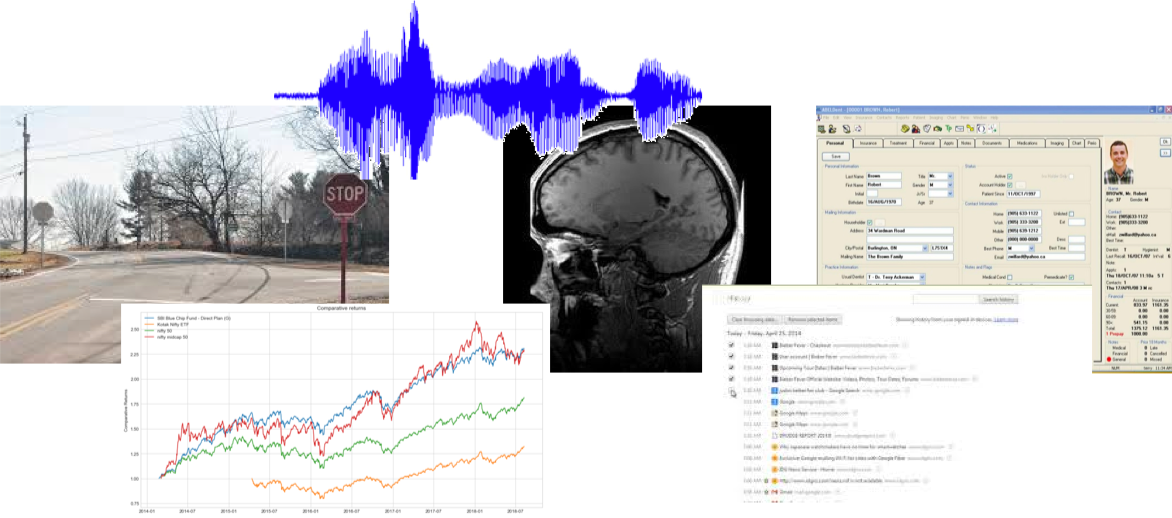
\includegraphics[width=.6\textwidth]{data_examples.png}
		\end{center}
		\item \textbf{Output:} A prediction or decision (this image is a stop sign, this stock will go up $10\%$ next quarter, turn the car right).
	\end{itemize}
\end{frame}

\begin{frame}
	\frametitle{classic example}
	\textbf{Optical character recognition (OCR)}: Decide if a handwritten character is an $a,b,\ldots, z, 0,1, \ldots, 9, \ldots$.
	\begin{center}
		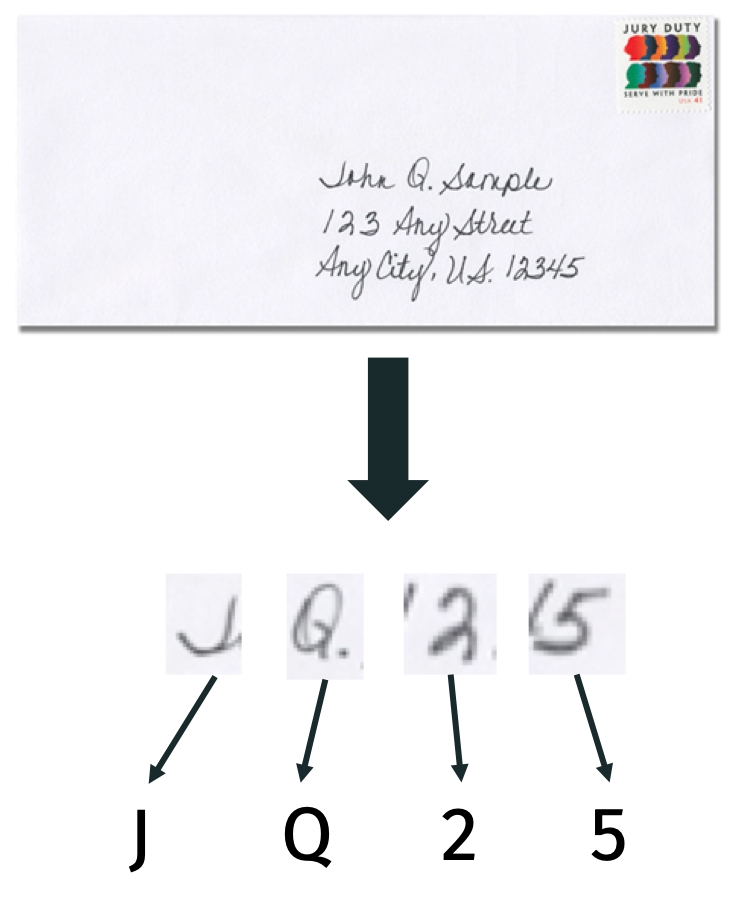
\includegraphics[width=.5\textwidth]{ocrPipeline.png}
	\end{center}
\end{frame}

\begin{frame}
	\frametitle{classic example}
	\textbf{Optical character recognition (OCR)}: Decide if a handwritten character is an $a,b,\ldots, z, 0,1, \ldots, 9, \ldots$.
	
	\textbf{Applications:}
	\begin{itemize}
		\item Automatic mail sorting.
		\item Text search in handwritten documents.
		\item Digitizing scanned books.
		\item License plate detection for tolls.
		\item Etc.
	\end{itemize}
\end{frame}

\begin{frame}[t]
	\frametitle{expert systems}
	How would you write an \textbf{algorithm} to distinguish these digits?
	\begin{center}
		
\includegraphics[width=.6\textwidth]{all_digits.png}
	\end{center}
	Suppose you just want to distinguish \emph{between a 1 and a 7}. 
\end{frame}

\begin{frame}
	\frametitle{1s vs. 7s  algorithm}
	\textbf{Reasonable approach:}
	A number which contains one vertical line is a $1$, if it contains one vertical and one horizontal line, it's a $7$.
	\begin{center}
		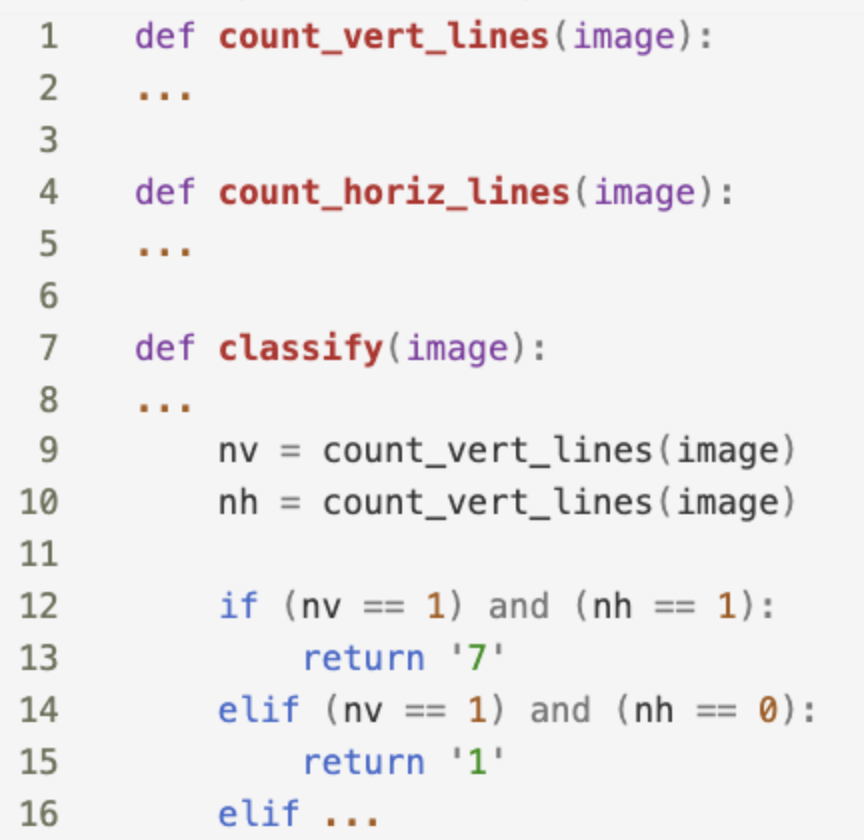
\includegraphics[width=.5\textwidth]{program.png}
	\end{center}
\end{frame}

\begin{frame}
	\frametitle{1s vs. 7s  algorithm}
	This rule breaks down in practice:
	\begin{center}
		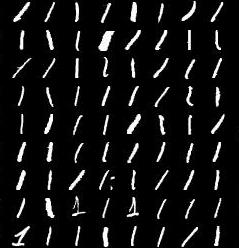
\includegraphics[width=.4\textwidth]{ones.jpg}\hspace{1em} 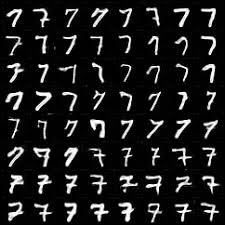
\includegraphics[width=.4\textwidth]{sevens.jpeg}
	\end{center}
	Even fixes/modifications of the rule tend to be brittle... Maybe you could get $80\%$ accuracy, but not nearly good enough.
\end{frame}

\begin{frame}
	\frametitle{challenge of expert systems}
	Rule based systems, also called \emph{Expert Systems} were \emph{the dominant approach} to artificial intelligence in the 70s and 80s.
	
	\vspace{1em}
	\textbf{Major limitation:} While human's are very good at many tasks,
	\begin{itemize}
		\item It's often hard to encode \emph{why} humans make decisions in simple programmable logic.
		\item We think in abstract concepts with no mathematical definitions (how exactly do you define a line? how do you define a curve? straight line?)
	\end{itemize}
\end{frame}

\begin{frame}
	\frametitle{a different approach: machine learning}
	Focus on what humans do well: solving the task at hand!

	\textbf{Step 1:}
	Collect and label many input/output pairs $(\bv{x}_i,y_i)$.
	For our digit images, we have each $\bv{x}_i\in \R^{28\times 28}$ and $y_i \in \{0, 1, \ldots, 9\}$. 
	\begin{center}
		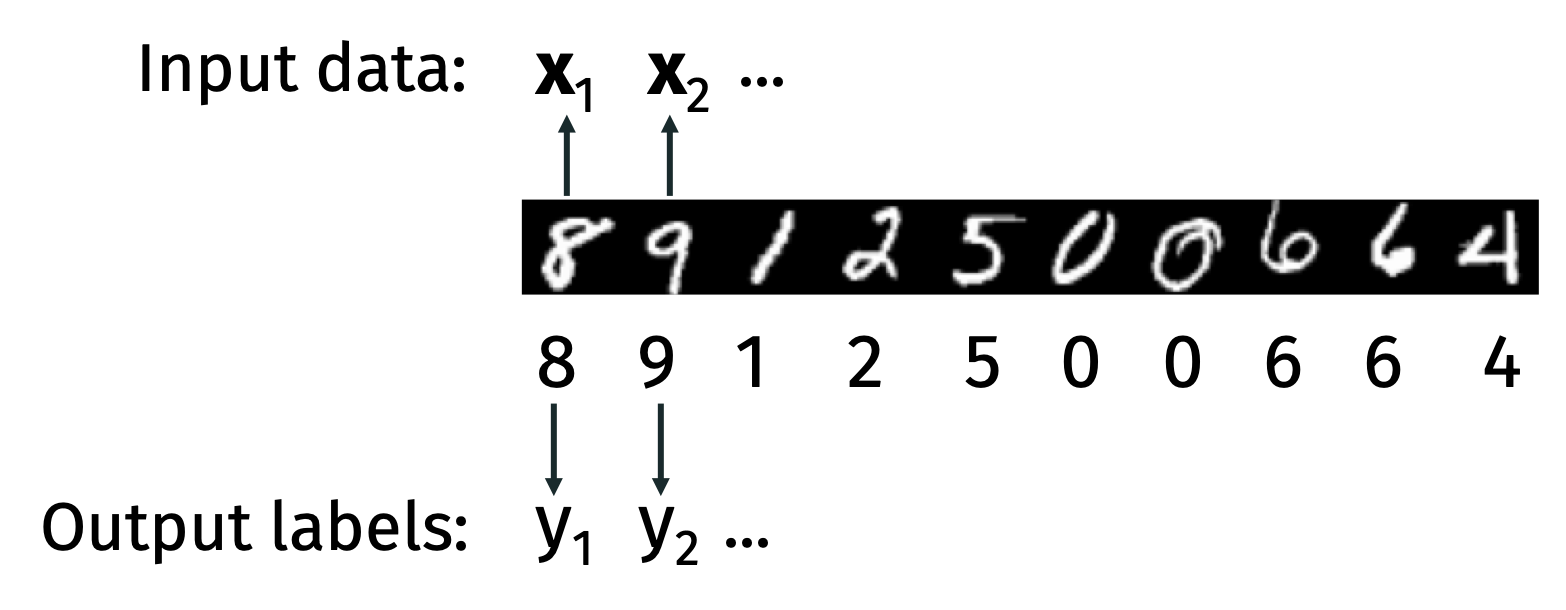
\includegraphics[width=.6\textwidth]{collect_data.png}
	\end{center}
	This is called the \textbf{\alert{training dataset.}}
\end{frame}

\begin{frame}
	\frametitle{a different approach: machine learning}
	\textbf{Step 2:} Learn from the examples we have.
	\begin{itemize}
		\item Have the computer \emph{automatically} find some function $f(\bv{x})$ such that $f(\bv{x}_i) = y_i$ for most $(\bv{x}_i,y_i)$ in our training data set (by searching over many possible functions).
	\end{itemize}
Think of $f$ as any crazy equation, or an arbitrary program:
\begin{align*}
f(\bv{x}) = 10 \cdot\bv{x}[1,1] - 6 \cdot\bv{x}[3,45]\cdot\bv{x}[9,99] + 5 \cdot\text{mean}(\bv{x}) + \ldots
\end{align*}


This approach of learning a function from \emph{labeled} data is called \alert{\textbf{supervised learning.}}
\end{frame}

\begin{frame}
	\frametitle{supervised learning for ocr}
	\small
	\emph{National Institute for Standards and Technology} collected a huge amount of handwritten digit data from census workers and high school students in the early 90s:
	\vspace{-1em}
	\begin{center}
		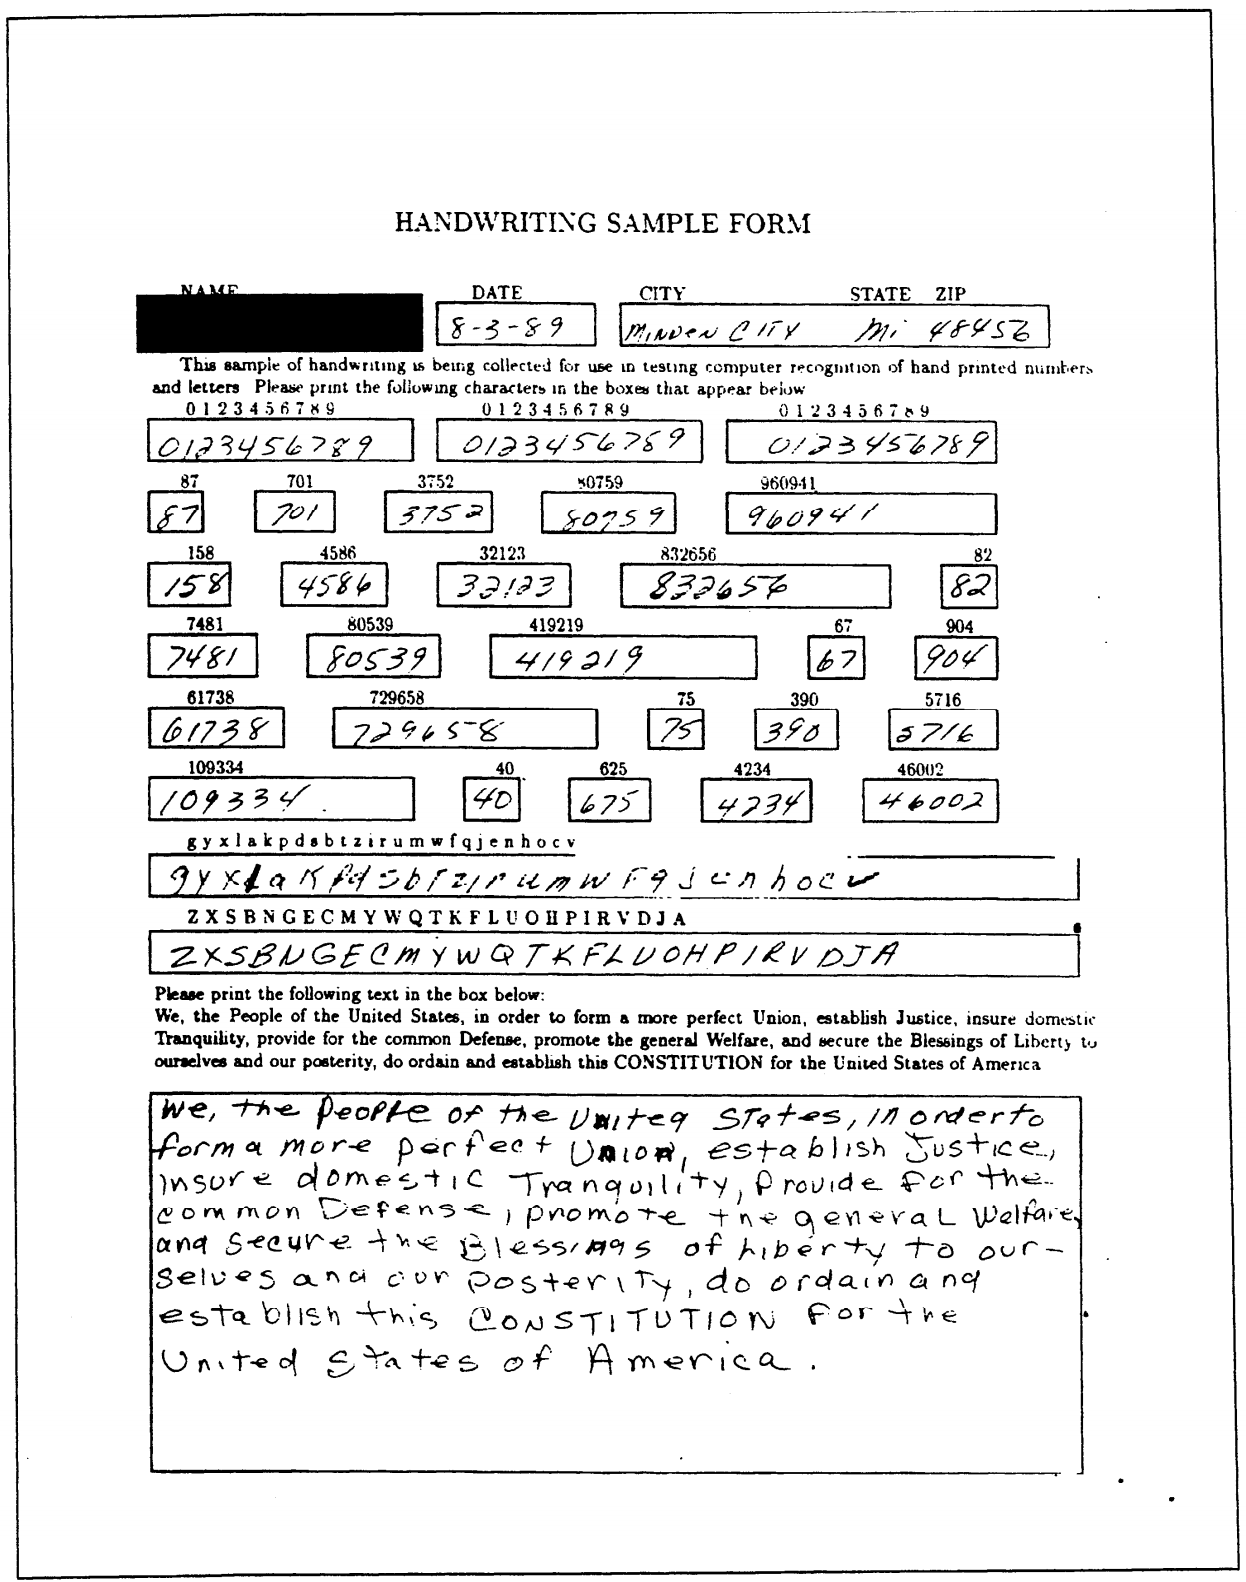
\includegraphics[width=.4\textwidth]{nist_data.png}
		
		This is called the NIST dataset, and was used to create the famous \textbf{\alert{MNIST handwritten digit dataset}}.
	\end{center}

\end{frame}

\begin{frame}
	\frametitle{machine learning}
	Since the 1990s machine learning have overtaken expert systems as the dominant approach to artificial intelligence.
	\begin{itemize}
		\item Current methods achieve $.21\%$ error rate for OCR on benchmark datasets (MNIST).
		\item Very successful on other problems as well. 
	\end{itemize}
\end{frame}

\begin{frame}
	\frametitle{modern machine learning}
	\begin{center}
	\textbf{\large You could not be studying ML at a more exciting time!}
	\end{center}
	
	\begin{columns}
		\begin{column}{.6\textwidth}
			\begin{itemize}
				\item Autonomous vehicles.
				\item Human level play in very difficult games. 
				\item Incredible machine translation.
				\item Pervasive impact in science and engineering.
				\item Many, many more.
			\end{itemize}
		\end{column}
		\begin{column}{.5\textwidth}
			\begin{center}
				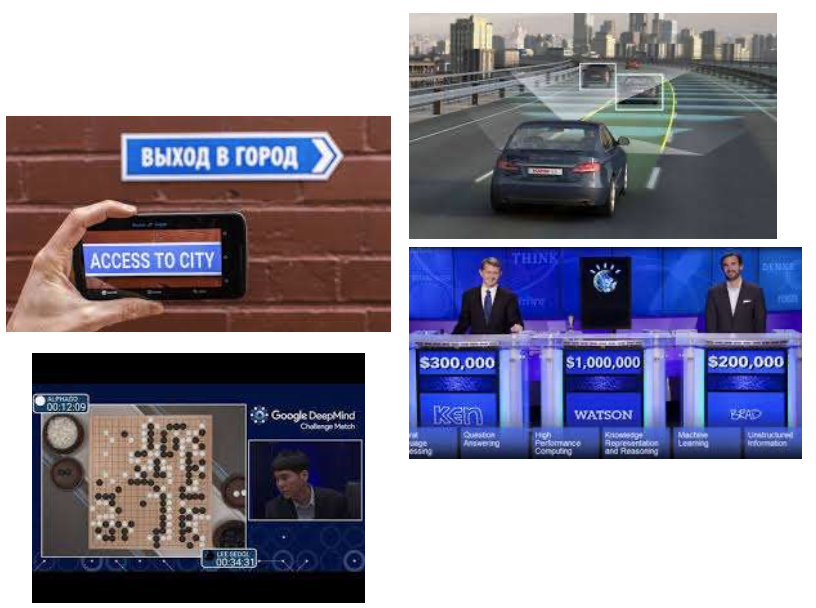
\includegraphics[width=\textwidth]{applications.png}
			\end{center}
		\end{column}
	\end{columns}
\end{frame}

\begin{frame}
	\frametitle{what is driving machine learning?}
	\textbf{Machine learning has benefited from an explosion in our ability to collect and store data}:
	\begin{itemize}
		\item Cheap, fast storage. Large data centers. 
		\item Pervasive monitoring (satellite imagery, cheap sensors, improved and reduced cost for technologies like LIDAR).
		\item Crowd-sourced data collection (images, text on the internet)
		\item Crowd-sourced data labeling via the internet (Amazon Mechanical Turk, reCAPTCHA, etc.)
	\end{itemize}
	\begin{center}
		\textbf{\alert{Having lots of data isn't enough. We have to know how to use it effectively.}}
	\end{center}
\end{frame}

\begin{frame}
	\frametitle{central questions in machine learning}
	Once we have the basic machine learning setup, many very difficult questions remain:
	\begin{itemize}
		\item How do we \alert{parameterize} a class of functions $f$ to search?
		\item How do we \alert{efficiently find} a good function in the class?
		\item How do we ensure that an $f(\bv{x})$ which works well on our training data will \alert{generalize} to perform well on future data? 
		\item How do we deal with \alert{imperfect data} (noise, outliers, incorrect training labels)?
	\end{itemize}
\end{frame}

\begin{frame}
	\frametitle{central questions in machine learning}
	In this course you will learn to answer these central questions through a combination of:
	\begin{itemize}
		\item \emph{Hands on implementation.}
		\begin{itemize}
			\item In-class demos and take-home labs using \texttt{Python} and \texttt{Jupyter notebooks}.
			\item Final Project (on any dataset/problem you like).
		\end{itemize}
		\item \emph{Theoretical exploration}. 
		\begin{itemize}
			\item Written problem sets.
			\item Two midterm exams.
		\end{itemize}
	\end{itemize}
\end{frame}

\begin{frame}
	\frametitle{course objectives}
	\textbf{Goals of hands-on component:}
	\begin{enumerate}
		\item Learn how to view and formulate real world problems in the language of machine learning. 
		\item Gain experience applying the most popular and most successful machine learning algorithms to example problems. The goal is to prepare you to use these tools in industrial or academic positions.
	\end{enumerate}
\end{frame}

\begin{frame}
	\frametitle{course objectives}
	\textbf{Goals of theoretical component:}
	\begin{enumerate}
		\item Learn how theoretical analysis can help explain the performance of machine learning algorithms and lead to the design of entirely new methods.
		\item Build experience with the most important mathematical tools used in machine learning, including probability, statistics, and linear algebra. This experience will prepare you for more advanced coursework in ML, or research. 
		\item Be able to understand contemporary research in machine learning, including papers from NeurIPS, ICML, ICLR, and other major machine learning venues. 
	\end{enumerate}
\end{frame}

%\begin{frame}
%	\frametitle{machine learning}
%	Types of \textbf{Supervised Learning:}
%	\begin{itemize}
%		\item \textbf{Classification} -- predict a \emph{discrete} class label.
%		\item \textbf{Regression} -- predict a \emph{continuous} value.
%	\end{itemize}
%\end{frame}
%
%\begin{frame}
%	\frametitle{supervised learning}
%	Another example of supervised classification: \textbf{Face Detection}.
%	\begin{center}
%		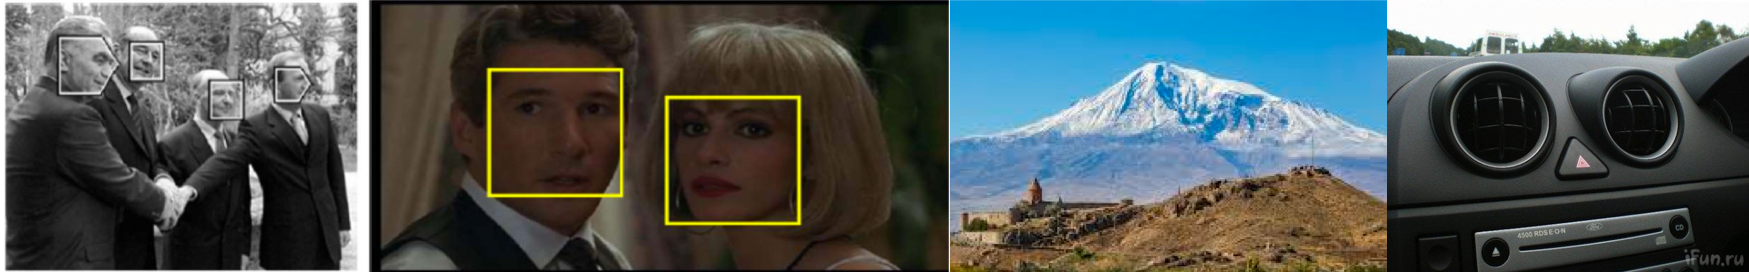
\includegraphics[width=.8\textwidth]{facedetection.png}
%	\end{center}
%	Each input $\bv{x}_i$ is an image. Each output $y_i$ is $1$ if the image contains a face, $0$ otherwise.
%	
%	\begin{itemize}
%		\item Harder than digit recognition, but we now have very reliable methods (used in nearly all digital cameras, phones, etc.)
%	\end{itemize}
%\end{frame}
%
%\begin{frame}
%	\frametitle{supervised learning}
%	Other examples of supervised classification:
%	\begin{itemize}
%		\item \emph{Object detection} (Input: image, Output: dog or cat)
%		\item \emph{Spam detection} (Input: email text, Output: spam or not)
%		\item \emph{Medical diagnosis} (Input: patient data, Output: disease condition or not)
%		\item \emph{Credit decision making} (Input: financial data, Output: offer loan or not)
%		\item Etc. 
%	\end{itemize}
%	
%\end{frame}
%
%\begin{frame}
%	\frametitle{supervised learning}
%	 Example of supervised regression: \textbf{Stock Price Prediction}.
%	\begin{center}
%		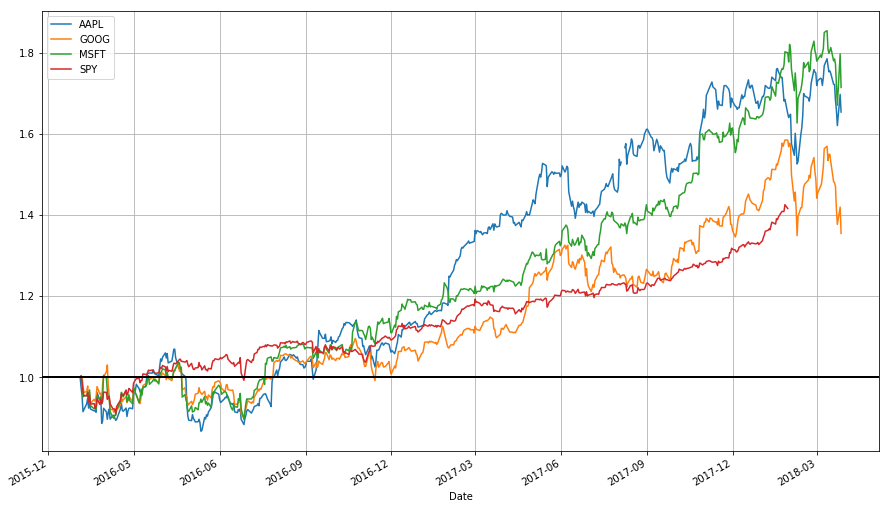
\includegraphics[width=.5\textwidth]{stock_data.png}
%	\end{center}
%	Each input $\bv{x}$ is a vector of metrics about a company (sales volume, PE ratio, earning reports, historical price data). 
%	
%	Each output $y_i$ is the price of the stock 3 months in the future. 
%\end{frame}
%
%\begin{frame}
%	\frametitle{supervised learning}
%	Other examples of supervised regression:
%	\begin{itemize}
%		\item \emph{Home price prediction} (Inputs: square footage, zip code, number of bathrooms)
%		\item \emph{Car price prediction} (Inputs: make, model, year, miles driven)
%		\item \emph{Weather prediction} (Inputs: weather data at nearby stations)
%		\item Etc.
%		
%	\end{itemize}
%\end{frame}
%
%\begin{frame}
%	\frametitle{other types of learning}
%	Later in the class we will talk about models beyond supervised learning: 
%	\begin{itemize}
%		\item Unsupervised learning
%		\item Reinforcement learning
%		\item Active learning
%	\end{itemize}
%\end{frame}

\begin{frame}
	\frametitle{basic information}
	All class information can be found at:
	\begin{center}
		\large \url{www.chrismusco.com/introml}
	\end{center}
\end{frame}


\end{document} 








